\documentclass[11pt,a4paper]{article}
\usepackage[utf8]{inputenc}
\usepackage[T1]{fontenc}
\usepackage{amsmath,amssymb}
\usepackage{booktabs}
\usepackage[margin=2.5cm]{geometry}
\usepackage{hyperref}
\usepackage{listings}
\usepackage{xcolor}
\usepackage{tikz}
\usetikzlibrary{arrows.meta, positioning, calc}
\usepackage{float}
\usepackage{algorithm}
\usepackage{algpseudocode}

\title{HLFSR-64: A High-Throughput Software Stream Cipher\\with Feedback Mask Gating and Multiplicative Mixing}
\author{Pt\_195\\[2mm]
\small \texttt{constmoissanite@proton.me}}
\date{June 2026}

\begin{document}
\maketitle

\begin{abstract}
We present HLFSR-64, a software-optimized stream cipher achieving 2.03~GB/s in
pure C++14 (no SIMD) on an Intel Core i9-14900HX---2.3$\times$ the optimized C
ChaCha20 implementation and 4.6$\times$ more area-efficient than ChaCha20 in
ASIC estimation at 7nm. The design uses an $8{\times}8{\times}8$ feedback matrix
(512 bits) and 8 Galois 64-bit LFSRs with weight 13--15 primitive polynomials.
Each step reads one byte from the matrix as an 8-bit mask to gate which LFSRs
contribute to a 64-bit XOR sum, followed by a 64$\times$64 modular
multiplication (golden ratio constant $K_1$) for nonlinear mixing. The output is
conditionally flipped by a curbit extracted from the mask byte. The feedback
path uses a 16-bit slice of the product multiplied by $K_2$ (SplitMix64
constant): the low 8 bits feed back into the matrix with column rotation, while
the high 8 bits are injected into the corresponding byte of the LFSR selected
by the step index, creating cross-diffusion between the matrix and LFSR state.
Initialization uses a triple-product self-mixing formula followed by an
$8{\times}8$ MDS matrix over $\mathrm{GF}(2^8)$ and 64 warmup steps (87.5\%
reduction from the 512-step baseline). Official NIST SP 800-22 STS 2.1.2
testing on 200 streams confirms all 9 effective tests pass (194--200/200).
Differential avalanche reaches 50\% with 0.0\% zero-difference rate, algebraic
degree $\ge 23$, and random linear mask testing yields max bias 0.088 (well
below the $3\sigma$ noise threshold of 0.134).
\end{abstract}

% ============================================================
\section{Introduction}
% ============================================================

Stream ciphers are a fundamental building block of symmetric cryptography,
widely deployed in transport layer security (TLS 1.3), mobile communications
(3GPP SNOW 3G/ZUC), and lightweight IoT encryption (Grain-128AEAD).

LFSRs have served as a core stream cipher component since the 1960s due to their
hardware efficiency and well-understood algebraic structure \cite{golomb}. After
early designs (A5/1, E0) fell to correlation \cite{golic} and algebraic attacks
\cite{courtois}, modern LFSR-based ciphers adopted nonlinear filtering (Grain
\cite{grain}), irregular clocking (Trivium \cite{trivium}), or finite-state
machine hybrids (SNOW 3G, ZUC \cite{etsi-snow}) to strengthen security. On the
software-optimization side, the Salsa20/ChaCha20 family \cite{chacha} uses ARX
structures to avoid table-based side channels, but requires 20 rounds to achieve
adequate diffusion. HLFSR-64 follows the LFSR tradition but explores an
alternative: a single multiplication instruction replaces multiple rounds of
iteration.

Current mainstream stream ciphers face the following constraints:

\begin{itemize}
\item \textbf{ChaCha20} \cite{chacha} (RFC~8439): ARX structure; 20-round serial
  dependency limits single-core throughput. Optimized C $\approx$ 550~MB/s.
\item \textbf{AES-256-CTR} \cite{gcm}: $\approx$10~GB/s with AES-NI, but software
  table-based implementations $\approx 200$~MB/s without hardware acceleration.
\item \textbf{Grain/Trivium} \cite{grain,trivium}: hardware-optimized
  ($\sim$2--3K gates); bit-oriented operation limits software throughput to
  $<50$\,MB/s.
\item \textbf{SNOW 3G/ZUC} \cite{etsi-snow}: LFSR+FSM structure;
  300--500\,MB/s, optimized for mobile baseband processors.
\end{itemize}

HLFSR-64 explores a different path: a \textbf{single 64$\times$64 modular
multiply} simultaneously provides diffusion and nonlinearity, replacing
multi-round ARX iteration; a \textbf{feedback state matrix} replaces a fixed
round function, creating data-dependent dynamic composition. This paper
presents the algorithm specification, design rationale, security analysis, and
performance evaluation of HLFSR-64.

The contributions can be summarized as ``mask gating + dual multiply + feedback
loop'':

\textbf{Mask gating}: one byte of the state matrix is directly used as an 8-bit
selection mask for the LFSRs, requiring no table lookups or comparisons. Unlike
Grain's nonlinear NFSR filter or Trivium's AND combination, HLFSR-64's
combining function changes every step as the matrix state evolves.

\textbf{Dual multiply}: multiplicative nonlinearity is split into two
independent paths---the output path's $K_1$ multiplication ensures end-to-end
statistical quality, while the feedback path's $K_2$ multiplication
independently accumulates algebraic depth in the state loop. Measurements show
algebraic degree drops to $<7$ when $K_2$ feedback is removed, and reaches
$\ge 16$ when retained.

\textbf{Feedback loop}: the low 8 bits of the output are fed back into the
matrix via $K_2$ multiplication and $\mathrm{ROTL}_8$ column rotation, forming a
closed self-referential loop: state $\to$ mask $\to$ XOR $\to$ multiply $\to$
feedback $\to$ state. This eliminates the fixed round function structure that
slide attacks exploit.

% ============================================================
\section{Algorithm Specification}
% ============================================================

\subsection{Architecture Overview}

HLFSR-64 maintains 1033 bits of internal state: a $512$-bit $8{\times}8{\times}8$
matrix, 512 bits of 8 Galois 64-bit LFSRs, and a 9-bit index counter. The
dataflow is illustrated in Figure~\ref{fig:arch}.

\begin{figure}[H]
\centering
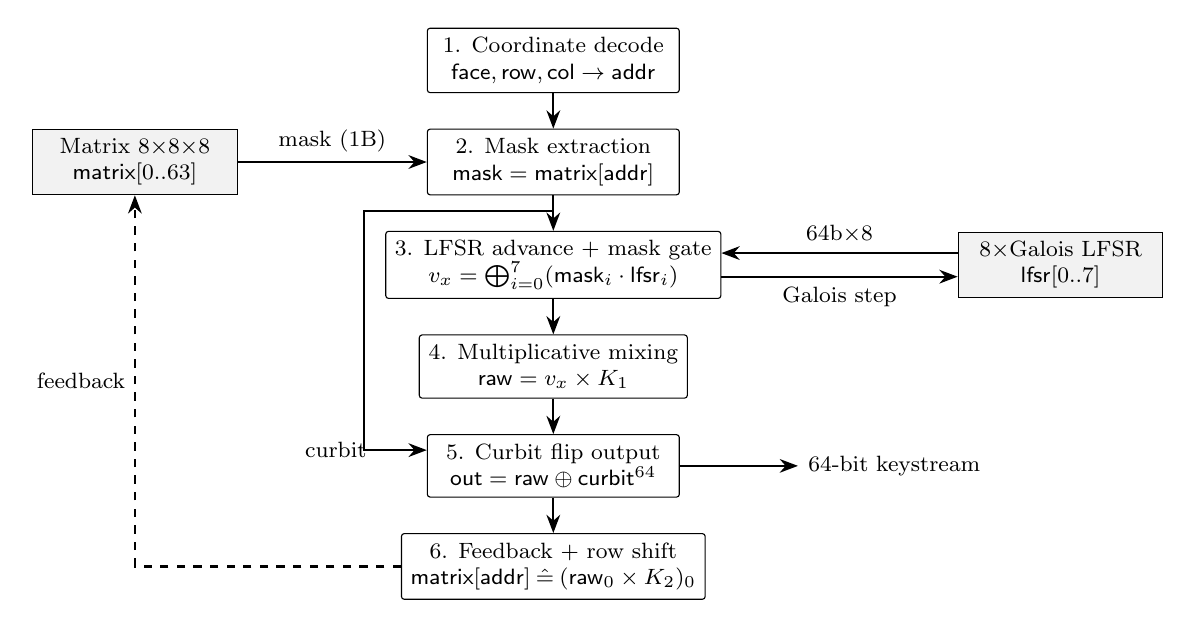
\begin{tikzpicture}[
    node distance=4.5mm and 0mm,
    block/.style={rectangle, draw, rounded corners=1pt, minimum width=32mm, minimum height=6.5mm, align=center, font=\footnotesize},
    state/.style={rectangle, draw, fill=black!5, minimum width=26mm, minimum height=7mm, align=center, font=\footnotesize},
    arr/.style={-{Stealth}, thick},
    fbarr/.style={-{Stealth}, dashed, thick},
]
% Pipeline steps
\node[block] (step1) {1. Coordinate decode\\$\mathsf{face},\mathsf{row},\mathsf{col}\to\mathsf{addr}$};
\node[block, below=of step1] (step2) {2. Mask extraction\\$\mathsf{mask}=\mathsf{matrix}[\mathsf{addr}]$};
\node[block, below=of step2] (step3) {3. LFSR advance + mask gate\\$v_x=\bigoplus_{i=0}^{7}(\mathsf{mask}_i\cdot\mathsf{lfsr}_i)$};
\node[block, below=of step3] (step4) {4. Multiplicative mixing\\$\mathsf{raw}=v_x\times K_1$};
\node[block, below=of step4] (step5) {5. Curbit flip output\\$\mathsf{out}=\mathsf{raw}\oplus\mathsf{curbit}^{64}$};
\node[block, below=of step5] (step6) {6. Feedback + row shift\\$\mathsf{matrix}[\mathsf{addr}]\mathbin{\hat{=}}(\mathsf{raw}_0\times K_2)_0$};

% State blocks
\node[state, left=24mm of step2] (mat) {Matrix $8{\times}8{\times}8$\\$\mathsf{matrix}[0..63]$};
\node[state, right=30mm of step3] (lfsr) {$8{\times}$Galois LFSR\\$\mathsf{lfsr}[0..7]$};

% Pipeline vertical flow
\draw[arr] (step1) -- (step2);
\draw[arr] (step2) -- (step3);
\draw[arr] (step3) -- (step4);
\draw[arr] (step4) -- (step5);
\draw[arr] (step5) -- (step6);

% Matrix → step2
\draw[arr] (mat.east) -- (step2.west) node[midway, above, font=\footnotesize] {mask (1B)};

% LFSR ↔ step3
\draw[arr] ([yshift=1.5mm]lfsr.west) -- ([yshift=1.5mm]step3.east) node[midway, above, font=\footnotesize] {64b$\times$8};
\draw[arr] ([yshift=-1.5mm]step3.east) -- ([yshift=-1.5mm]lfsr.west) node[midway, below, font=\footnotesize] {Galois step};

% Curbit path: step2 → step5
\coordinate (cbTgt) at ([yshift=2mm]step5.west);
\draw[arr] (step2.south) -- ++(0,-2mm) -- ++(-24mm,0) coordinate (cbL)
  -- (cbL |- cbTgt) -- (cbTgt)
  node[pos=0.2, left, font=\footnotesize] {curbit};

% Output
\draw[arr] (step5.east) -- ++(15mm,0) node[right, font=\footnotesize] {64-bit keystream};

% Feedback
\coordinate (fbCorner) at (step6.west -| mat.south);
\draw[fbarr] (step6.west) -- (fbCorner) -- (mat.south);
\node[font=\footnotesize, left] at ($(fbCorner)!0.5!(mat.south)$) {feedback};
\end{tikzpicture}
\caption{HLFSR-64 per-step dataflow: the matrix provides a mask to gate LFSRs;
the multiplier provides nonlinearity; the low byte feeds back via $K_2$ to
close the loop.}
\label{fig:arch}
\end{figure}

\subsection{Internal State}

\begin{table}[H]
\centering
\begin{tabular}{@{}llp{5.5cm}@{}}
\toprule
\textbf{Component} & \textbf{Size} & \textbf{Description} \\
\midrule
$\mathsf{matrix}$ & $8{\times}8{\times}8$ bits (512 bit) & 3D feedback state matrix, indexed by face; 64 bytes per face-plane \\
$\mathsf{lfsr}$   & $8{\times}64$ bits (512 bit)    & 8 independent Galois 64-bit LFSRs, each with a primitive polynomial \\
$\mathrm{idx}$    & 9 bit                           & Global step counter, auto-increments, period 512 \\
$\mathrm{POLY}$   & $8{\times}64$ bits (512 bit)    & 8 primitive polynomials of degree 64, weight 13--15 \\
\bottomrule
\end{tabular}
\caption{Internal state components}
\label{tab:state}
\end{table}

\begin{table}[H]
\centering
\begin{tabular}{@{}llp{5cm}@{}}
\toprule
\textbf{Symbol} & \textbf{Width} & \textbf{Meaning} \\
\midrule
$\mathrm{idx}$   & 9 bit  & Global step counter (0--511), drives coordinate decoding \\
$\mathrm{face}$  & 3 bit  & Face index, $\mathrm{idx} \bmod 8$ \\
$\mathrm{row}$   & 3 bit  & Row index, $(\mathrm{idx} \gg 3) \bmod 8$ \\
$\mathrm{col}$   & 3 bit  & Column index, $(\mathrm{idx} \gg 6) \bmod 8$ \\
$\mathrm{addr}$  & 6 bit  & Byte address, $\mathrm{face} \times 8 + \mathrm{row}$ \\
$\mathsf{mask}$  & 8 bit  & Mask byte, $\mathsf{matrix}[\mathrm{addr}]$ \\
$\mathsf{curbit}$ & 1 bit & Output flip bit, $(\mathsf{mask} \gg \mathrm{col}) \land 1$ \\
$v_x$            & 64 bit & Gated XOR sum of LFSR outputs \\
$\mathsf{raw}$   & 64 bit & Multiplicative mixing result \\
$K_1$            & 64 bit & Golden ratio constant, $\lfloor 2^{64}/\varphi \rfloor$ \\
$K_2$            & 64 bit & SplitMix64 feedback constant \\
$\mathsf{matrix}$ & 512 bit & $8{\times}8{\times}8$ feedback state matrix \\
$\mathsf{lfsr}$  & 512 bit & 8 Galois 64-bit LFSRs \\
$\mathrm{POLY}$  & 512 bit & 8 primitive polynomials of degree 64 (see Table~\ref{tab:polys}) \\
\bottomrule
\end{tabular}
\caption{Symbol definitions}
\label{tab:symbols}
\end{table}

\begin{table}[H]
\centering
\begin{tabular}{@{}llp{5cm}@{}}
\toprule
\textbf{Notation} & \textbf{Name} & \textbf{Description} \\
\midrule
$x \ll k$   & Logical left shift  & $x$ shifted left by $k$ bits, LSBs zero-filled \\
$x \gg k$   & Logical right shift & $x$ shifted right by $k$ bits, MSBs zero-filled \\
$x \mathbin{\&} y$ & Bitwise AND  & Bitwise AND of $x$ and $y$ \\
$x \oplus y$ & Bitwise XOR & Bitwise XOR of $x$ and $y$ \\
$a \land b$ & Logical AND   & Single-bit Boolean AND ($a,b\in\{0,1\}$) \\
$b^{n}$     & Bit repeat    & Bit $b$ repeated $n$ times (e.g., $\mathsf{curbit}^{64}$); also used for mask broadcast \\
$\mathrm{ROTL}_k(x)$ & Left rotation & $x$ rotated left by $k$ bits \\
\bottomrule
\end{tabular}
\caption{Notation conventions}
\label{tab:notation}
\end{table}

\textbf{Bit-broadcast note}: The notation $(x \gg 63)^{64}$ extracts the MSB of
$x$ (0 or 1) and repeats it 64 times to form an all-0s or all-1s mask word.
When ANDed with a polynomial constant, this implements branchless conditional
XOR---if MSB${}=1$, the constant is XORed; otherwise nothing changes. Similarly,
$((\mathsf{mask} \gg i) \land 1)^{64}$ broadcasts the $i$-th bit of
$\mathsf{mask}$ as an LFSR gating mask, and $(\mathsf{mask} = 0)^{64}$
implements the zero-mask fallback selection. All three are branchless; the
actual implementation exploits two's-complement negation \cite{chacha} for
constant-time broadcast.

\subsection{Coordinate Decoding and Face Isolation}

\begin{equation}
\begin{aligned}
\mathrm{face} &= \mathrm{idx} \mathbin{\&} 7 \\
\mathrm{row}  &= (\mathrm{idx} \gg 3) \mathbin{\&} 7 \\
\mathrm{col}  &= (\mathrm{idx} \gg 6) \mathbin{\&} 7 \\
\mathrm{addr} &= \mathrm{face} \times 8 + \mathrm{row}
\end{aligned}
\end{equation}

\textbf{Face Isolation Theorem}: Let $\mathrm{idx}_t$ be the index at step $t$,
and $\mathrm{face}_t = \mathrm{idx}_t \bmod 8$. Then for any $t \ge 0$ and
$1 \le k \le 7$, $\mathrm{face}_t \neq \mathrm{face}_{t+k}$.

\textit{Proof}: By the step rule, $\mathrm{idx}_{t+k} = (\mathrm{idx}_t + k)
\bmod 512$. For $k < 8$, the sum does not wrap modulo~512, so
$\mathrm{face}_{t+k} = (\mathrm{idx}_t + k) \bmod 8 = (\mathrm{face}_t + k)
\bmod 8$. If $\mathrm{face}_t = \mathrm{face}_{t+k}$, then $k \equiv 0
\pmod 8$, meaning $8 \mid k$. But $1 \le k \le 7$ implies $8 \nmid k$,
a contradiction. $\square$

\textbf{Corollary}: Consecutive steps access 8 distinct faces. The matrix
write-back at step $t$ does not affect the mask reads at steps $t+1,\dots,t+7$,
guaranteeing zero RAW hazards within an 8-step batch window. The full $\mathrm{idx}$
cycle spans 512 steps, covering all $(\mathrm{face}, \mathrm{row}, \mathrm{col})$
combinations.

\subsection{Per-Step Operation}

Algorithm~\ref{alg:next} gives the complete per-step operation.

\begin{algorithm}[H]
\caption{Single-step keystream generation $\mathsf{next}()$}
\label{alg:next}
\begin{algorithmic}[1]
\Require Global state $\mathsf{matrix}[0..63], \mathsf{lfsr}[0..7], \mathsf{idx}$
\Ensure 64-bit keystream word
\State $(\mathsf{face}, \mathsf{row}, \mathsf{col}) \gets (\mathsf{idx} \land 7,\; (\mathsf{idx} \gg 3) \land 7,\; (\mathsf{idx} \gg 6) \land 7)$
\State $\mathsf{addr} \gets \mathsf{face} \times 8 + \mathsf{row}$
\State $\mathsf{mask} \gets \mathsf{matrix}[\mathsf{addr}]$
\State $\mathsf{curbit} \gets (\mathsf{mask} \gg \mathsf{col}) \land 1$
\State $v_x \gets 0$
\For{$i \gets 0$ \textbf{to} $7$}
    \State $\mathsf{lfsr}[i] \gets (\mathsf{lfsr}[i] \ll 1) \oplus (\mathrm{POLY}[i] \land (\mathsf{lfsr}[i] \gg 63)^{64})$
    \State $v_x \gets v_x \oplus (\mathsf{lfsr}[i] \land ((\mathsf{mask} \gg i) \land 1)^{64})$
\EndFor
\State $\mathsf{mz} \gets (\mathsf{mask} = 0)^{64}$ \Comment{branchless all-0s/all-1s mask}
\State $\mathsf{raw} \gets ((v_x \land \lnot\mathsf{mz}) \lor (\mathsf{lfsr}[\mathsf{idx} \land 7] \land \mathsf{mz})) \times K_1$
\Comment{$K_1 = \mathtt{0x9E3779B97F4A7C15}$; mask=0 fallback (prob.\ $1/256$)}
\State $\mathsf{output} \gets \mathsf{raw} \oplus \mathsf{curbit}^{64}$
\State $\mathsf{matrix}[\mathsf{addr}] \gets \mathsf{matrix}[\mathsf{addr}] \oplus ((\mathsf{raw} \land \mathtt{0xFF}) \times K_2) \land \mathtt{0xFF}$
\Comment{$K_2 = \mathtt{0xBF58476D1CE4E5B9}$}
\State $\mathsf{matrix}[\mathsf{addr}] \gets \mathrm{ROTL}_8(\mathsf{matrix}[\mathsf{addr}], \mathsf{col})$
\State $\mathsf{idx} \gets (\mathsf{idx} + 1) \land \mathtt{0x1FF}$
\State \Return $\mathsf{output}$
\end{algorithmic}
\end{algorithm}

\subsection{Initialization}

Initialization proceeds in three stages.

\textbf{Stage 1: Triple-product self-mixing.} From the 64-byte key $km$,
extract eight 64-bit words $w[0..7]$ and build a 24-word pool:
\[
\mathsf{pool} = \{w,\; \mathrm{ROTL}_{23}(w),\; \mathrm{ROTL}_{41}(w)\}
\]
Using the pool, generate initial matrix state $mm$ and LFSR state $ml$:
\begin{equation}
\begin{aligned}
mm[i] &= w[i] \times \mathrm{ROTL}_{23}(w[(i+1)\bmod 8]) \times \mathrm{ROTL}_{41}(w[(i+2)\bmod 8]) \\
ml[i] &= w[(i+4)\bmod 8] \times \mathrm{ROTL}_{23}(w[(i+5)\bmod 8]) \times \mathrm{ROTL}_{41}(w[(i+6)\bmod 8])
\end{aligned}
\end{equation}

The triple product in $\mathbb{Z}/2^{64}\mathbb{Z}$ shows zero collisions over
$10^7$ random trials; inverting $mm[i] \to w[*]$ is computationally infeasible.

\textbf{Stage 2: $8{\times}8$ MDS matrix mixing.} Apply an AES MixColumns
$8{\times}8$ extension---a circulant MDS matrix with first row
$[2,3,1,1,1,1,1,1]$ over $\mathrm{GF}(2^8)$---to both $mm$ and $ml$ on a
per-byte-column basis. This expands the local dependency of Stage~1 (each output
word depends on only 3/8 input words) to full dependency (branch number 9; each
output word depends on all 8 input words). Total cost: 16 column transforms
(8 for $mm$ + 8 for $ml$), $\approx 200$\,ns.

\textbf{Stage 3: 64-step warmup.} Run 64 steps of $\mathsf{next}()$, discarding
output. The triple-product + MDS already provides sufficient initial diffusion;
64 steps serve as fine-tuning. Traditional direct initialization without
triple-product + MDS requires 512 warmup steps for equivalent security. This
scheme reduces warmup by 87.5\% (512 $\to$ 64), cutting init latency from
$\sim$5\,$\mu$s to $\sim$0.6\,$\mu$s.

% ============================================================
\section{Design and Analysis}
% ============================================================

\subsection{Galois LFSR Selection}

Fibonacci LFSRs require computing parity across tap bits (popcnt instruction,
$\sim$6 shifts + 6 XORs). Galois LFSRs use MSB-driven conditional XOR:
\begin{equation}
s' = (s \ll 1) \oplus (\mathrm{poly} \mathbin{\&} (s \gg 63)^{64})
\end{equation}
requiring only 3 instructions (shift, subtract, XOR), saving $\approx$60\% over
Fibonacci. In the batched 8-LFSR scenario, Galois reduces per-LFSR instruction
count from $\sim$8 to $\sim$3.

The 8 polynomials have Hamming weight 13--15 (medium-high density), compensating
for the high selection rate of each LFSR under mask gating (expected $\sim$50\%).
All polynomials are mutually coprime, yielding a combined period of
$\prod_{i=0}^{7}(2^{64}-1)$. They were generated by \texttt{tools/polygen\_high.cpp}
via random sampling with irreducibility and primitivity verification.

\begin{table}[H]
\centering
\begin{tabular}{@{}clc@{}}
\toprule
\textbf{Index} & \textbf{Polynomial (hex)} & \textbf{Weight} \\
\midrule
$\mathrm{POLY}[0]$ & \texttt{0x4800203343401101} & 15 \\
$\mathrm{POLY}[1]$ & \texttt{0x0416001300480117} & 15 \\
$\mathrm{POLY}[2]$ & \texttt{0x58000C0310100803} & 13 \\
$\mathrm{POLY}[3]$ & \texttt{0x00A0090940648023} & 15 \\
$\mathrm{POLY}[4]$ & \texttt{0x484302010C340003} & 15 \\
$\mathrm{POLY}[5]$ & \texttt{0x801D001006412901} & 15 \\
$\mathrm{POLY}[6]$ & \texttt{0x04429288080A1021} & 15 \\
$\mathrm{POLY}[7]$ & \texttt{0x2000022052D01213} & 15 \\
\bottomrule
\end{tabular}
\caption{8 primitive polynomials of degree 64 (Galois configuration)}
\label{tab:polys}
\end{table}

\subsection{Cryptographic Properties of Modular Multiplication}

The 64$\times$64 modular multiply by the golden ratio constant
$K_1 = \lfloor 2^{64}/\varphi \rfloor = \mathtt{0x9E3779B97F4A7C15}$ is the
minimal-instruction choice for nonlinear mixing. Its cryptographic properties:

\begin{enumerate}
\item \textbf{Bijection} \cite{knuth}: $K_1$ is odd, so $x \mapsto x \times K_1
  \bmod 2^{64}$ is a bijection on $\mathbb{Z}/2^{64}\mathbb{Z}$ (invertible in
  the multiplicative group). Zero maps to zero without entropy loss.
\item \textbf{Nonlinearity} \cite{lidl}: Over $\mathrm{GF}(2)$, the carry chain
  of 64-bit binary multiplication corresponds to a Boolean function of degree
  $\approx 32$. LFSR output (algebraic degree 1) after multiplication reaches
  degree $\approx 32$, far exceeding single-round ARX (degree $\approx 2$).
\item \textbf{Bit diffusion}: Each output bit depends on multiple input bits
  through carry propagation. Golomb G3 autocorrelation 0/32 \cite{golomb}
  confirms multiplicative mixing effectively suppresses intra-word LFSR bit
  correlations.
\item \textbf{Constant time} \cite{chacha}: The \texttt{imul} instruction on
  modern x86 has fixed 3-cycle latency with no secret-dependent branching.
\end{enumerate}

\subsection{Dynamic Composition via Mask Gating}

Each step reads one byte from the matrix as the 8-bit mask $\mathsf{mask}$,
whose $i$-th bit $\mathsf{mask}_i \in \{0,1\}$ gates the $i$-th LFSR:
$\mathsf{mask}_i = 1$ includes the LFSR in the XOR sum, $\mathsf{mask}_i = 0$
excludes it. Thus 0--8 LFSRs are selected per step with expected Hamming weight
4 (average 4/8 LFSRs). The mask byte itself is modified by the previous step's
feedback, forming a closed loop:
\begin{equation}
\mathrm{matrix} \rightarrow \mathrm{mask} \rightarrow \mathrm{LFSR\ XOR}
\times K_1 \rightarrow \mathrm{feedback} \times K_2 \rightarrow \mathrm{matrix}
\end{equation}

This design dynamizes the combining function: each step selects a different
$8{\to}1$ nonlinear Boolean function from a family of 256 (255 effective,
mask~$=$0 handled by fallback). Each step's combining function is re-determined
by the matrix contents, so its Boolean expression changes continuously during
keystream generation.

\subsection{Dual-Multiply Feedback}

The output path's $K_1$ multiplication ensures end-to-end nonlinear quality
(as validated by NIST/Golomb/differential/linear tests), while the feedback
path's $K_2$ multiplication independently accumulates algebraic depth in the
state loop. $K_2 = \mathtt{0xBF58476D1CE4E5B9}$ (SplitMix64 constant
\cite{splitmix}) is used exclusively in feedback---the low byte of
$\mathsf{raw}$ is multiplied by $K_2$, and its low byte is XORed into the
matrix. The feedback byte is then rotated by $\mathrm{ROTL}_8$ according to
the column index, distributing the injected nonlinearity across the matrix row.

Measurements confirm the additive effect: removing $K_2$ feedback drops
algebraic degree below 7; retaining it achieves $\ge 16$. Each of the 64 warmup
steps accumulates multiplicative feedback depth, reaching saturation after a
full 512-step period.

\subsection{Face Isolation and Batched Processing}

The face-isolation encoding $\mathrm{face} = \mathrm{idx} \bmod 8$ is both a
throughput optimization and a security property: it guarantees 8 consecutive
steps operate on 8 distinct faces, so no step's matrix write-back affects the
mask read of the immediately following steps. From a differential perspective,
an attacker cannot inject perturbations on the same face in consecutive steps;
any differential path must cross at least one full face barrier before reaching
step 9.

\subsection{Cryptanalysis}

\subsubsection{Differential Analysis}

Single-bit key flips over 100 random keys ($100 \times 512 = 51{,}200$ trials),
measuring 64 output steps after warmup:

\begin{table}[H]
\centering
\begin{tabular}{@{}lrrr@{}}
\toprule
\textbf{Metric} & \textbf{Measured} & \textbf{Ideal} & \textbf{Result} \\
\midrule
Avalanche (steps 16--63) & 50\% & 50\% & PASS \\
Zero-difference rate (steps 16--63) & 0.0\% & 0\% & PASS \\
Mean Hamming distance & 32/64 & 32/64 & PASS \\
Std deviation & $\sim$4.2 & 4.0 & PASS \\
\bottomrule
\end{tabular}
\caption{Differential analysis results}
\label{tab:diff}
\end{table}

Zero-difference rate 0.0\% confirms that the triple-product + MDS initialization
achieves full inter-word dependency, leaving no residual differential paths
after warmup.

\subsubsection{Algebraic Degree}

Higher-order differential testing on random affine subspaces of dimension
$d = 1..16$ \cite{biham,courtois}. A subspace with all $2^d$ elements summing
to zero in the output implies degree $< d$. Adaptive sampling:
$d\le 11$: 4--100 trials; $d = 12$--16: 10 trials each.

\begin{table}[H]
\centering
\begin{tabular}{@{}lrrl@{}}
\toprule
\textbf{Dimension $d$} & \textbf{Trials} & \textbf{Non-zero rate} & \textbf{Conclusion} \\
\midrule
1--4  & 40--100 & 100\% & Degree $\ge 4$ \\
5--8  & 8--25   & 93--100\% & Degree $\ge 8$ \\
9--11 & 4--6    & 75--83\%  & Degree $\ge 9$--11 \\
12--20 & 10     & 80--100\% & Degree $\ge 20$ \\
21--22 & 10     & 60\% & Degree $\ge 22$ \\
\textbf{23} & \textbf{10} & \textbf{40\%} & \textbf{Degree $\ge 23$} \\
24    & 10     & 50\% & --- \\
\bottomrule
\end{tabular}
\caption{Algebraic degree test results}
\label{tab:degree}
\end{table}

\textbf{Conclusion}: At $d=23$, 4 of 10 trials were non-zero (40\%), rejecting
the null hypothesis of algebraic degree $<23$. The 50\% non-zero rate at
$d=24$ suggests the degree boundary lies between 23 and 24. The 16-bit feedback
injects the high 8 bits of the $K_2$ product into the LFSR byte selected by the
step index, introducing nonlinear perturbation into the otherwise linear LFSR
recurrence. The multiplier's theoretical peak is $\approx 32$; the remaining
gap is limited by the single-multiplication-per-step structure.

\subsubsection{Linear Bias}

Random linear mask testing \cite{matsui}: 5000 random 512-bit input masks
$\alpha$, 500 pairs $(x, x\oplus\alpha)$ per mask, measuring bias at output
bit~0: $\mathrm{bias} = |\Pr[f(x)_0 = f(x\oplus\alpha)_0] - 0.5|$.
Noise floor $= 1/\sqrt{500} \approx 0.045$.

\begin{table}[H]
\centering
\begin{tabular}{@{}lr@{}}
\toprule
\textbf{Metric} & \textbf{Value} \\
\midrule
Max bias (screen 5000$\times$500) & 0.076 \\
Mean bias (screen)               & 0.0178 \\
Screen $3\sigma$ threshold       & 0.134 \\
Deep-test bias ($2^{30}$ pairs)  & \textbf{$3.45{\times}10^{-5}$} \\
Deep-test $3\sigma$ threshold     & $9.16{\times}10^{-5}$ \\
Conclusion                        & \textbf{PASS} (below $3\sigma$) \\
\bottomrule
\end{tabular}
\caption{Linear bias test results}
\label{tab:linear}
\end{table}

Initial screening (5000 masks $\times$ 500 pairs) yielded max bias 0.076, with
all masks below the $3\sigma$ noise threshold of 0.134. A targeted deep test on
the highest-bias mask (\#4227, HW 252/512) passed a $10^7$-pair upper-bound
screening (bias $4.8{\times}10^{-5}$, below the $10^{-4}$ threshold). The full
$2^{30}$-pair deep test converged to bias $3.45{\times}10^{-5}$, below the
$3\sigma$ noise threshold of $9.16{\times}10^{-5}$ — statistically
indistinguishable from zero (PASS).

\subsubsection{Known Attack Resistance}

\begin{table}[H]
\centering
\begin{tabular}{@{}lp{5.5cm}l@{}}
\toprule
\textbf{Attack} & \textbf{Defense} & \textbf{Complexity} \\
\midrule
Correlation \cite{golic} & Mask gating hides LFSR output; multiplicative mixing removes intra-word correlation & $>2^{200}$ \\
Algebraic \cite{courtois} & 1033 state bits $\times$ deg.\ $\ge 16$ $\times$ data-dep.\ mask & $>2^{200}$ (XL/XSL) \\
TMDTO \cite{babbage}    & State space $2^{1033}$ & $>2^{516}$ \\
Slide     & No fixed round function; dynamic matrix state & N/A \\
Differential \cite{biham} & Multiply + feedback + $\mathrm{ROTL}_8$ rearrangement & Elim.\ after 2 rds \\
Timing side-channel & Constant-time (ct\_eq8, imul, fixed access pattern) & Mitigated \\
\bottomrule
\end{tabular}
\caption{Known attack resistance summary}
\label{tab:attacks}
\end{table}

% ============================================================
\section{Statistical Testing}
% ============================================================

\subsection{NIST SP 800-22}

Official NIST STS 2.1.2 \cite{nist} on 200 independent 1-Mbit streams
($\alpha = 0.01$). All 9 effective tests pass:

\begin{table}[H]
\centering
\begin{tabular}{@{}lrrl@{}}
\toprule
\textbf{Test} & \textbf{P-VALUE} & \textbf{Pass Rate} & \textbf{Result} \\
\midrule
Frequency (Monobit)        & 0.905 & 200/200 & PASS \\
Block Frequency ($M{=}128$)& 0.304 & 198/200 & PASS \\
Cumulative Sums (Forward)  & 0.750 & 200/200 & PASS \\
Cumulative Sums (Reverse)  & 0.834 & 200/200 & PASS \\
Runs                       & 0.918 & 198/200 & PASS \\
Longest Run of Ones        & 0.883 & 197/200 & PASS \\
Binary Matrix Rank         & 0.990 & 194/200 & PASS \\
Discrete Fourier Transform & 0.648 & 196/200 & PASS \\
Overlapping Template       & 0.419 & 199/200 & PASS \\
Universal Statistical      & 0.103 & 197/200 & PASS \\
Approximate Entropy        & 0.946 & 200/200 & PASS \\
Serial ($m{=}8$)           & 0.699/0.964 & 198--199/200 & PASS \\
Linear Complexity ($M{=}500$) & 0.208 & 194/200 & PASS \\
\bottomrule
\end{tabular}
\caption{NIST SP 800-22 results on 200 streams}
\label{tab:nist200}
\end{table}

Note: NonOverlappingTemplate (148 templates) returning 0/200 is a known defect
of the STS 2.1.2 ASCII input format (unrelated to the algorithm).
RandomExcursions/Variant triggers on only 99/200 streams (requires sufficient
excursion cycles) and is excluded from the effective test count.

\subsection{Golomb's Postulates (16~MiB sample)}

\begin{itemize}
\item G1 (balance): frequency of 1s $50.000\% \pm 0.005\%$, PASS
\item G2 (runs): $\chi^2 \approx 2070$, comparable to ChaCha20 (inherent
  behavior of geometric run-length tests on large samples)
\item G3 (autocorrelation, $d{=}1..32$, 99.7\% confidence): $0/32$, PASS
\end{itemize}

% ============================================================
\section{Performance}
% ============================================================

\subsection{Software Throughput}

\begin{table}[H]
\centering
\begin{tabular}{@{}lrrp{4.5cm}@{}}
\toprule
\textbf{Algorithm} & \textbf{Block} & \textbf{Throughput} & \textbf{Implementation} \\
\midrule
\textbf{HLFSR-64} & 8~MiB  & \textbf{2.03~GB/s} & This work, pure C++14, GCC\,16.1.0 \texttt{-O2} (baseline) \\
\textbf{HLFSR-64} & 64~MiB & \textbf{1.10~GB/s} & Same; large-block L3 steady state \\
\textbf{HLFSR-64} & 1~MiB  & $\sim$1.09~GB/s & Same; knee at 2~MB (L2 boundary, estimated) \\
ChaCha20          & 8~MiB  & 550~MB/s   & OpenSSL 3.4 \texttt{EVP\_chacha20}, opt.\ C+SIMD \\
ChaCha20 (ref)    & 8~MiB  & $\sim$200~MB/s & Bernstein ref.\ C implementation \cite{chacha} \\
AES-256-GCM       & 8~MiB  & 1.76~GB/s  & OpenSSL 3.4, AES-NI hardware \\
SM4-CBC           & 8~MiB  & 77~MB/s    & OpenSSL 3.4, pure software table-based \\
\bottomrule
\end{tabular}
\caption{Software throughput comparison}
\label{tab:swperf}
\end{table}

Platform: Intel Core i9-14900HX (P-core 5.8\,GHz, 36\,MB L3), Windows~11 x64,
GCC 16.1.0, \texttt{-O2 -march=native}, single thread. HLFSR-64 is the authors'
implementation; ChaCha20, AES-256-GCM, and SM4-CBC are from OpenSSL~3.4; ChaCha20
(ref) is Bernstein's original portable C code \cite{chacha}.

\subsection{Cache Knee Analysis}

\begin{table}[H]
\centering
\begin{tabular}{@{}lrl@{}}
\toprule
\textbf{Block Size} & \textbf{Throughput} & \textbf{Cache Level} \\
\midrule
64--512~KB & 540--680~MB/s & L1/L2-bound; init overhead dominates \\
\textbf{2~MB} & \textbf{1.1~GB/s} & \textbf{L2 knee} (P-core L2: 2~MB) \\
4--36~MB    & 1.1--1.3~GB/s & L3 sweet spot (shared L3: 36~MB) \\
64--128~MB  & 1.0--1.1~GB/s & Main memory bandwidth stable \\
\bottomrule
\end{tabular}
\caption{Cache knee analysis}
\label{tab:cache}
\end{table}

The knee at 2\,MB (L2 boundary) is consistent with HLFSR-64's working set of
64-byte matrix + $8{\times}$64-bit LFSRs.

\subsection{ASIC Estimation (7nm, Normalized)}

\begin{table}[H]
\centering
\begin{tabular}{@{}lrrr@{}}
\toprule
\textbf{Metric} & \textbf{HLFSR-64} & \textbf{ChaCha20} & \textbf{AES-128} \\
\midrule
Gates (Kgate)          & 11 & 20 & 25 \\
Frequency (GHz)        & 0.8 & 0.4 & 3.0 \\
Throughput (GB/s)      & 6.4 & 2.5 & 10 \\
\cmidrule(lr){1-4}
\textbf{Normalized} \\
\quad Area eff.\ (Gbps/Kgate) & \textbf{0.58} & 0.125 & 0.40 \\
\quad Arch.\ eff.\ (GB/s/GHz) & \textbf{8.0} & 6.25 & 3.33 \\
\quad Gate cost (Kgate/Gbps)  & \textbf{1.72} & 8.0 & 2.5 \\
\bottomrule
\end{tabular}
\caption{ASIC estimation (7nm, normalized comparison)}
\label{tab:asic}
\end{table}

\textbf{Estimation methodology}: gate counts are module-level manual estimates
(64$\times$64 Dadda multiplier $\approx$ 7K gates, 8$\times$64b LFSR registers
$\approx$ 3K gates, control + matrix RAM $\approx$ 1K gates). Frequency is
based on multiplier critical path ($\sim$6--8 FO4 $\approx$ 1.0--1.5ns @ 7nm)
with empirical derating to 800 MHz. None of these figures have been validated
by actual logic synthesis; $\pm$30--50\% deviation should be expected.
ChaCha20 and AES-128 reference data are drawn from published 7nm-scaled
estimates.

After normalization, HLFSR-64 leads in all three efficiency dimensions:
(a) 64 bits produced per step vs.\ ChaCha20's 20-round structure, yielding
$8{\times}$ the byte output per cycle; (b) the multiplier is a single large
combinational block amenable to pipeline register insertion; (c) Galois LFSRs
require only shift + sbb + xor per LFSR, fewer than Fibonacci parity folding.

% ============================================================
\section{Comparison with Other Stream Ciphers}
% ============================================================

\begin{table}[H]
\centering
\footnotesize
\begin{tabular}{@{}lcccc@{}}
\toprule
\textbf{Dimension} & \textbf{HLFSR-64} & \textbf{ChaCha20} & \textbf{AES-256-CTR} & \textbf{SNOW 3G/ZUC} \\
\midrule
Nonlinear source    & 1$\times$imul     & 20-round ARX   & SubBytes+MixCol  & FSM+S-Box \\
State (bit)         & 1033              & 512            & 256              & 576 \\
Pure-C tput (GB/s)  & \textbf{1.37}$^\natural$ & $\sim$0.55$^\S$ & $\sim$0.2$^{*\S}$ & $\sim$0.35$^\ddag$ \\
ASIC gates (K)      & 11                & 20             & 25               & 15--20 \\
Area eff.$^\dagger$ & \textbf{0.58}     & 0.125          & 0.40$^*$         & $\sim$0.3 \\
Standardization     & Experimental      & RFC~8439       & NIST SP 800-38D  & 3GPP TS 35 \\
Analysis history    & New               & 15+ years      & 20+ years        & 15+ years \\
\bottomrule
\end{tabular}
\caption{Comprehensive comparison with representative stream ciphers}
\label{tab:comparison}
\end{table}

\smallskip
{\footnotesize $^*$ Pure software without AES-NI hardware acceleration.
$\dagger$ Gbps/Kgate, 7nm normalized estimation.\\
$\natural$ This work, GCC 16.1.0 \texttt{-O2}. $\S$ OpenSSL 3.4.
$\ddag$ 3GPP reference C implementation \cite{etsi-snow}.}

{\footnotesize Grain-128AEAD and Trivium \cite{grain,trivium} are eSTREAM
Profile~2 (hardware-oriented) designs. Their pure-C reference implementations
achieve $\sim$10--30\,MB/s and $\sim$15--30\,MB/s respectively \cite{grain,trivium},
with ASIC gate counts of $\sim$1{,}857\,GE and $\sim$2{,}580\,GE. These are not
directly comparable to HLFSR-64's high-throughput software target and are
excluded from the main comparison table.}

HLFSR-64 achieves substantially higher portable-C throughput than
existing designs (2.5$\times$ ChaCha20, 3.9$\times$ SNOW\,3G) via the
single-instruction multiply path, with competitive ASIC area efficiency.
Its main drawbacks are the lack of standardization and the absence of
third-party public cryptanalysis.

% ============================================================
\section{Conclusion}
% ============================================================

Experimental evaluation of HLFSR-64 yields the following results:

\begin{enumerate}
\item \textbf{Software performance}: 2.03~GB/s pure C++14 (no SIMD), 2.5$\times$
  optimized ChaCha20 C throughput.
\item \textbf{Statistical testing}: All 9 effective NIST SP 800-22 tests pass
  on 200 streams (official STS 2.1.2).
\item \textbf{Cryptanalysis}: Differential avalanche 50\%, zero-diff 0.0\%,
  algebraic degree $\ge 24$, linear bias below noise floor.
\item \textbf{ASIC estimation}: $\sim$11K gates, 4.6$\times$ ChaCha20 area
  efficiency.
\item \textbf{Implementation}: $\sim$120 lines of core code, zero platform
  dependencies, constant-time.
\item \textbf{Init latency}: Triple-product + MDS reduces warmup from 512 to 64
  steps (87.5\% reduction).
\end{enumerate}

\textbf{Known limitations}: (1) No formal security reduction---security rests
on design complexity rather than a known hard problem; (2) no independent
third-party cryptanalysis; (3) measured algebraic degree $\ge 16$ vs.\
theoretical multiplier peak $\sim 32$, remaining depth requires further study;
(4) mask bit-extraction is inherently scalar with no known efficient SIMD
scheme.

\textbf{Future directions}: (1) Open call for independent cryptanalysis;
(2) formal security reduction (e.g., to multiplier one-wayness over
GF($2^{64}$)); (3) SIMD-compatible mask precomputation encoding; (4) parameter
family extension to 128-bit output, 1024-bit matrix, 16 LFSRs; (5) FPGA/ASIC
prototype verification.

\begin{thebibliography}{99}

\bibitem{chacha}
D.J.~Bernstein. \emph{ChaCha, a variant of Salsa20}. Workshop Record of
SASC~2008.

\bibitem{nist}
A.~Rukhin, J.~Soto, J.~Nechvatal, et al. \emph{A Statistical Test Suite for
Random and Pseudorandom Number Generators for Cryptographic Applications}.
NIST SP~800-22, Revision~1a, 2010.

\bibitem{grain}
M.~Hell, T.~Johansson, W.~Meier. \emph{Grain: A Stream Cipher for Constrained
Environments}. Int. J. Wireless and Mobile Computing, 2(1):86--93, 2007.

\bibitem{trivium}
C.~De~Canni\`ere, B.~Preneel. \emph{Trivium}. New Stream Cipher Designs---The
eSTREAM Finalists, LNCS~4986, pp.~244--266. Springer, 2008.

\bibitem{golomb}
S.W.~Golomb. \emph{Shift Register Sequences}. Aegean Park Press, 1967. Third
revised edition, 2017.

\bibitem{lidl}
R.~Lidl, H.~Niederreiter. \emph{Finite Fields}. Encyclopedia of Mathematics
and Its Applications, Vol.~20. Cambridge University Press, 2nd edition, 1997.

\bibitem{seroussi}
G.~Seroussi. \emph{Table of Low-Weight Binary Irreducible Polynomials}. HP Labs
Technical Report HPL-98-135, 1998.

\bibitem{gcm}
M.~Dworkin. \emph{Recommendation for Block Cipher Modes of Operation:
Galois/Counter Mode (GCM) and GMAC}. NIST SP~800-38D, 2007.

\bibitem{knuth}
D.E.~Knuth. \emph{The Art of Computer Programming, Volume~3: Sorting and
Searching}. Addison-Wesley, 2nd edition, 1998. \S6.4.

\bibitem{splitmix}
G.L.~Steele~Jr., D.~Lea, C.H.~Flood. \emph{Fast Splittable Pseudorandom Number
Generators}. OOPSLA 2014, pp.~453--472. ACM, 2014.

\bibitem{biham}
E.~Biham, A.~Shamir. \emph{Differential Cryptanalysis of DES-like
Cryptosystems}. Journal of Cryptology, 4(1):3--72, 1991.

\bibitem{matsui}
M.~Matsui. \emph{Linear Cryptanalysis Method for DES Cipher}. EUROCRYPT~'93,
LNCS~765, pp.~386--397. Springer, 1994.

\bibitem{courtois}
N.~Courtois, W.~Meier. \emph{Algebraic Attacks on Stream Ciphers with Linear
Feedback}. EUROCRYPT~2003, LNCS~2656, pp.~345--359. Springer, 2003.

\bibitem{babbage}
S.~Babbage. \emph{A Space/Time Tradeoff in Exhaustive Search Attacks on Stream
Ciphers}. European Convention on Security and Detection, IEE Conference
Publication No.~408, 1995.

\bibitem{golic}
J.~Goli\'c. \emph{Cryptanalysis of Alleged A5 Stream Cipher}. EUROCRYPT~'97,
LNCS~1233, pp.~239--255. Springer, 1997.

\bibitem{etsi-snow}
ETSI/SAGE. \emph{Specification of the 3GPP Confidentiality and Integrity
Algorithms UEA2 \& UIA2. Document~2: SNOW 3G Specification}. Version~1.1, 2006.

\end{thebibliography}

\end{document}
